\chapter{Literature Review}
\label{ch:literaturereview_report}

In order to tackle the research questions, different disciplines of software engineering such as Complex datasets, Compiler reporting, Continuous integration, Refactoring tools, Issue tracker, Stack Overflow, Gamification, Usability Engineering are looked into and studied what ideas we can adapt into our scenario along with own novel solution ideas. \\ \\

After doing the literature review in the disciplines mentioned above, there are a few essential takeaways in the scope of this thesis. In the area of ‘Complex datasets’, Dix et al. \cite{Dix} with their current research talks about more complex grouping and linking of datasets in the context of a user interface of Spreadsheets application. There could be two datasets with fields having a similar meaning and fields that are entirely different. So, the key takeaway is about design lessons of extensibility of columns. For example, ‘venues were geocoded to allow spatial graphs’ could be related as dates in bug reports to some standard format. It is done for all tools used and then shown on a unified interface. Next, Gaur et al. \cite{Gaur} speaks about the linear search problem in indexing as it takes more time for large volumes of data. So, different parameters are introduced to decrease computation time. For example, it linearly searches a database with toys.  It takes more time than a modified query like ‘a toy in red colour and horse types’.  By looking at two parameters, i.e., colour and type simplifies the search. This analogy sparks the idea of grouping bugs as per module, bug type, which could ease user in finding a particular bug on an interface. \\ \\

In the area of ‘Compiler reporting’, Horning et al. \cite{horning} mentions the importance of error logging with statistics as to what the compilers are expected to tell the user. It also mentions the importance of stating what kind of bugs does the tool did not find along with bugs found, but in reality, this questions the scalability. So, the key takeaway is that it is ideal for showing the number of specific bugs founds in an analysis. Next in the area of ‘Refactoring tools’, Dustinca \cite{dustinca} talks about how these tools are to be built and in user context, it has to overcome the barrier of discoverability which means the difficulty of use. To assist the developer on this issue, they introduced a smart tag in the context of the user editor and notified which parts of the code we can refactor. This analogy emphasises the importance of ‘on-board’ phase, which plays a vital role in the gamification \cite{gamify} discipline. Hayashi et al. \cite{Hayashi} illustrate the importance of task-level commits in order to maintain an edit history of refactoring. This concept gives an idea of which a user does a bug-fix level commit to addressing the traceability scenario. Mealy et al. \cite{Mealy} mentions about the importance of usability for software refactoring tools, and this could perhaps give some basic guidelines similar to knowing Usability Engineering \cite{usability} discipline. \\ \\

In the area of ‘Issue tracker’, Baysal et al. \cite{Baysal} mentions reducing the information overload for a developer in using the issue tracker. It is found out in their research paper that there is too much of information they receive. It confuses the developer in how to react, for example, the developer receives a high number of bugs reported via email, and this leads to a situation where the developer ignore the email. They found some exciting solution ideas, such as having a private dashboard for each developer as it becomes easy to react to issues corresponding to them. Expressiveness is one other mentioned in their paper, which says an example, severity or priority are vague terms to describe a bug. Perhaps it is ideal to describe the priory as per team decision instead of personal choice. This approach signifies in categorising the results as per categories in our unified interface. Next in ‘Stack Overflow’, in a research paper by Wang et al. \cite{stack} it is found there are 10934198 questions on a ‘User Interface’ topic, for example. It is quite challenging to go through such a high volume database. However, the Stack Overflow team has a friendly user interface, as shown in the following \autoref{fig:stackoverflow}. It uses some clean filter techniques such as tags for each topic, priority and trending. A research by Treude et al. \cite{Treude.2011} found out that most of the questions (72.30\%) in Stack Overflow have between 2 and 4 tags. This approach could perhaps ease in filtering/indexing issues. \\ \\

\begin{figure}[hbt!]
	\centering
	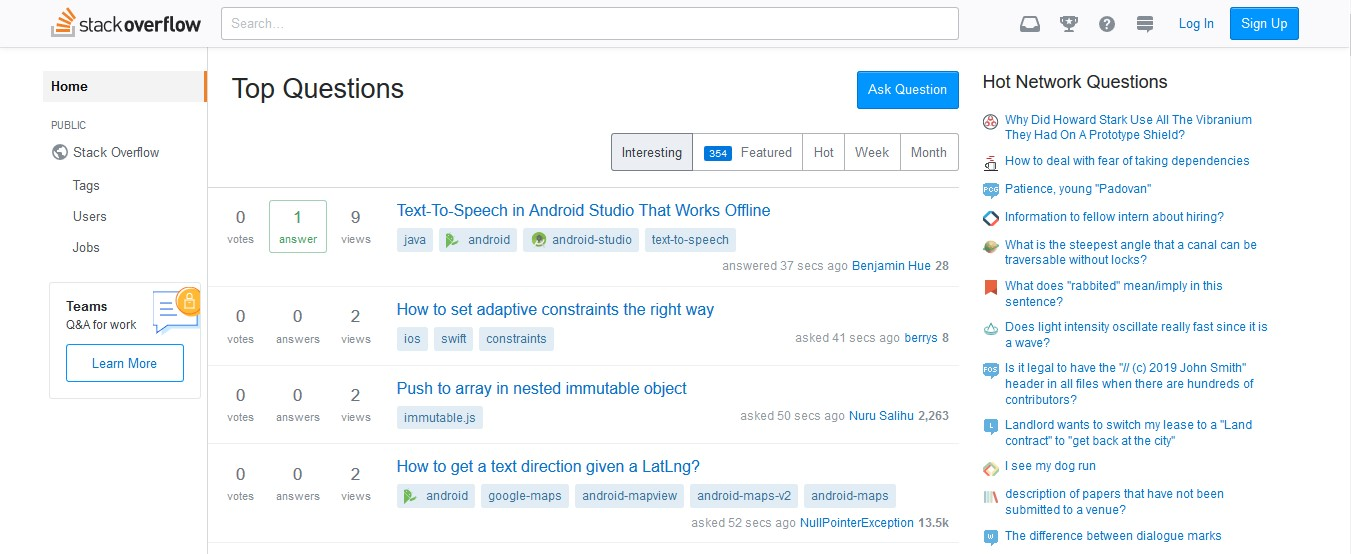
\includegraphics[width=\linewidth]{figures/stackoverflow}
	\caption{An user interface of Stack Overflow Website. \cite{stackoverflow}}
	\label{fig:stackoverflow}
\end{figure}